\documentclass[11pt, a4paper]{article}

\usepackage[margin=1in]{geometry}
\usepackage{microtype}
\usepackage{lmodern}
\usepackage{listings}
\usepackage{float}
\usepackage{enumitem}
\usepackage{xcolor}
\usepackage{tikz}
\usetikzlibrary{automata, positioning, arrows.meta}

\usepackage{caption}
\captionsetup[lstlisting]{labelformat=empty, skip=1pt, font=it, size=footnotesize}
\captionsetup[table]{labelformat=empty, skip=1pt, font=it, size=footnotesize}

\lstset{
    basicstyle=\ttfamily\footnotesize,
    keywordstyle=\color{blue}\bfseries,
    commentstyle=\color{green!50!black},
    stringstyle=\color{purple},
    frame=single,
    framerule=0.1pt,
    showstringspaces=false,
    captionpos=b,
    morekeywords={function, locals, entry, const, cast,
un, bin, addr_of, member_ptr, load, store, call, jump, cjump, return, void, ptr, true, false,
null, to, extern, type, bool, i32, i64, u32, f64}
}

\title{\textbf{CPS2000 Assignment Report}}
\author{Daniel Vella 0147005L}
\date{\today}

\begin{document}

\maketitle


\section{Introduction}
In this report I will start by delving into how my compiler is structured, focusing on one file at a time,
since each file directly reflects the tasks as defined in the assignment specification. Then I will discuss the testing suite
by showing the expected outcome of the tests found in the source code, and also how the compiler can be run on any sfile of source code.

\section{Compiler Structure}
The compiler was implemented in the OCaml language, using dune as the build system. I chose to use this language because
I realised when conducting my preliminary research that the project would require a lot of enumeration and comparison, for example to deduce
what token a certain string forms. This is something that OCaml handles very elegantly through its variant type definition 
and \texttt{match\dots with} pattern-matching construct. Also dune allows for the setup and management of the testing suite
to be kept separate from the main code implementation, while still being simple to run and update.

\medskip

Each file discussed in the following subsections implements the required task in the last defined function in the file using all the
previous type definitions and helper functions to achieve that.

\subsection{Task 1 - lexer.ml}
The natural first step of the Lexer is defining the tokens as a new type, allowing me to pattern match an incoming character or string onto a token. 
Below is an example of part of the type definition, and how it is used in part of the \texttt{map\_keywords} function:

\medskip

\begin{lstlisting}[language={[Objective]Caml}]
type token = 
(* Structure and Declaration *)
Extern | Type | Function | Locals | Void | Entry | To |
(* Instruction *)
Const | Cast | Un | Bin | Addr_Of | Member_Ptr | Load | Store | Call | 
Jump | Cjump | Return | ...

let map_keywords s = 
    match s with
    | "extern" -> Extern | "type" -> Type | "function" -> Function 
    | "locals" -> Locals | "void" -> Void | "entry" -> Entry 
    | "to" -> To | "const" -> Const | "cast" -> Cast | "un" -> Un 
    | "bin" -> Bin | "addr_of" -> Addr_Of | ... 
\end{lstlisting}

\medskip

For the purpose of the lexer the operator keywords, such as \texttt{add, sub, neg,\dots}
were not defined as tokens themselves, but instead consumed as Idents after the \texttt{Un} or 
\texttt{Bin} tokens, since they are not reserved words according to the assignment specification. 
Every other expected keyword or punctuation defined in the grammar of the ResIR language has its own assigned token, with some having implicit types, 
such as \texttt{Ident of string} and \texttt{IntLit of int}. Notably, \texttt{Local of string} allows
for a Local to be tokenized as a single item rather than having to carry a percent token and an Ident token into the parser.

\medskip

The same is true for the \texttt{Label of string}, but this is not something the DFSA can resolve itself, 
since something like \texttt{bb10} is handled as an Ident. Instead this is resolved when mapping states onto tokens,
using the \texttt{is\_numeric} and \texttt{is\_label} functions, which check if the Ident is of the Label
form \texttt{'bb' Digit \{Digit\}}.

\medskip

A \texttt{chars} type and a \texttt{states} type were defined to make the transition table more readable.
Rather than the table being full of seemingly random numbers, instead it cleanly indicates what character
will cause which transition, with the only added overhead being the simple \texttt{map\_char, st\_int, ch\_int}
functions. This then allows for the \texttt{map\_states} function to assign the correct token to a respective lexeme
based on the state that the transition table stopped at, including easy error checking as shown below:

\medskip

\begin{lstlisting}[language={[Objective]Caml}]
let map_states state lexeme line col = 
    let err_prefix = 
        Printf.sprintf "Lexical Error at Line %d, Col %d: " line col in
    match state with 
    | IdentSt -> if is_label lexeme then Label lexeme else map_keywords lexeme
    ...
    (* incomplete token states *)
    | StartSt -> failwith (err_prefix ^ "Empty Token")
    | PercentSt -> 
        failwith (err_prefix ^ "Standalone '%' symbol. Expected an identifier.")
    | PlusSt -> 
        failwith (err_prefix ^ "Standalone '+' symbol. Expected a literal. 
            Did you mean 'add'?")
    ...
\end{lstlisting}

\medskip

The only deviation from the supplied grammar in this section is that I decided to allow 
positive number literals, such as \texttt{+45}, so an extra state is needed in the transition table.
A benefit of this is that it allows for a more clear error message when something like \texttt{22 + 33}
is found by the Lexer, as shown in the code above. Below is the DFSA implemented by the transition table
in \texttt{lexer.ml}, where every missing state transition is mapped onto the Error state:

\medskip

\begin{figure}[H]
    \centering
    \resizebox{0.78\textwidth}{!}{
    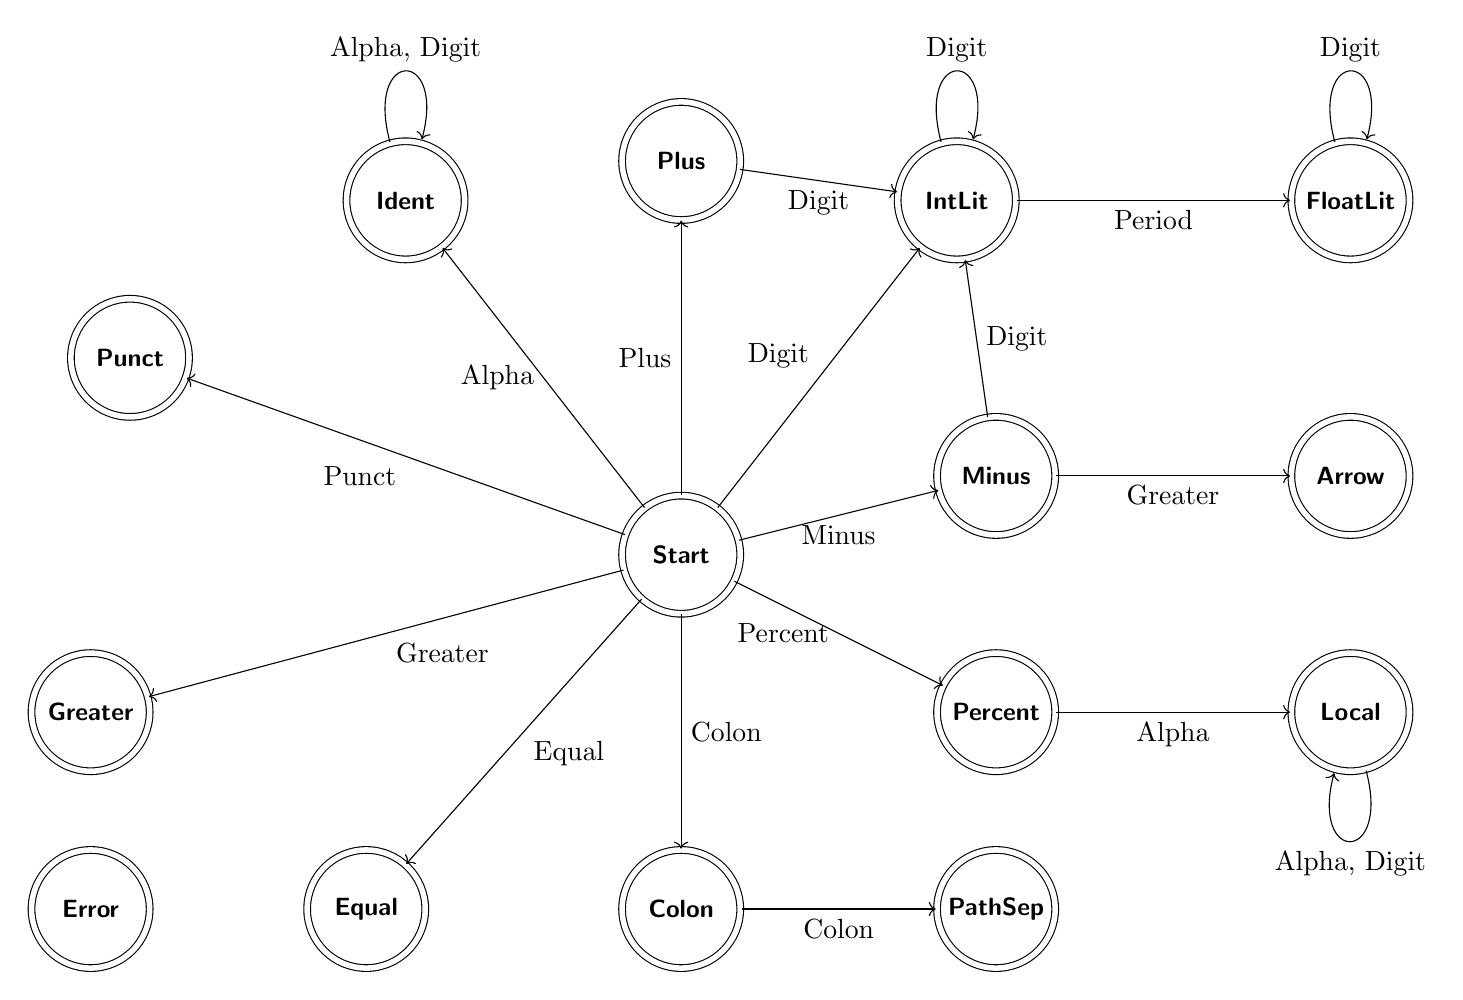
\begin{tikzpicture}[
        ->, % Uses clean modern arrowheads
        auto,
        % --- Customize Your Sizing Globally Right Here ---
        every state/.style={
            minimum size=1.5cm,        % Diameter of all circles
            inner sep=2pt,             % Text padding
            font=\small\sffamily\bfseries, % Clean, bold font style matching the image
            double distance=2pt
        },
        every edge/.style={draw, thin}
    ]

    % ==================== 1. STATE DEFINITIONS ====================
    % Center Point
    \node[state] (start) at (0,0) {Start};

    % Top Layer (Left to Right)
    \node[state, accepting] (ident)    at (-3.5, 4.5)  {Ident};
    \node[state]            (plus)     at (0, 5)       {Plus};
    \node[state, accepting] (intlit)   at (3.5, 4.5)   {IntLit};
    \node[state, accepting] (floatlit) at (8.5, 4.5)   {FloatLit};

    % Middle Right Layer
    \node[state]            (minus)    at (4, 1)       {Minus};
    \node[state, accepting] (arrow)    at (8.5, 1)     {Arrow};

    % Bottom Right Layer
    \node[state]            (percent)  at (4, -2)      {Percent};
    \node[state, accepting] (local)    at (8.5, -2)    {Local};

    % Bottom Layer (Right to Left)
    \node[state, accepting] (pathsep)  at (4, -4.5)    {PathSep};
    \node[state, accepting] (colon)    at (0, -4.5)    {Colon};
    \node[state, accepting] (equal)    at (-4, -4.5)   {Equal};
    \node[state] (error)    at (-7.5, -4.5) {Error};
    
    % Middle Left Layer
    \node[state, accepting] (greater)  at (-7.5, -2)   {Greater};
    \node[state, accepting] (punct)    at (-7, 2.5)    {Punct};

    \path 
        % Radiating Outward from Start
        (start) edge node[left] {Alpha}   (ident)
                edge node[left]        {Plus}    (plus)
                edge node[above left]  {Digit}   (intlit)
                edge node[below]       {Minus}   (minus)
                edge node[left] {Percent} (percent)
                edge node[right]        {Colon}   (colon)
                edge node[below right] {Equal}   (equal)
                edge node[below right]       {Greater} (greater)
                edge node[below left]       {Punct}   (punct)

        % Inter-State Connections
        (plus)    edge node[below] {Digit}   (intlit)
        (minus)   edge node[right]        {Digit}   (intlit)
                  edge node[below]       {Greater} (arrow)
        (intlit)  edge node[below]       {Period}  (floatlit)
        (percent) edge node[below]       {Alpha}   (local)
        (colon)   edge node[below]       {Colon}   (pathsep)

        % Self Loops (Above States)
        (ident)    edge [loop above] node {Alpha, Digit} (ident)
        (intlit)   edge [loop above] node {Digit}        (intlit)
        (floatlit) edge [loop above] node {Digit}        (floatlit)
        (local) edge [loop below] node {Alpha, Digit} (local);

    \end{tikzpicture}
    }
\end{figure}

\medskip

The Lexer makes use of the above tools to collect tokens by using the transition table to move
to the next state until the next state is the ErrorState, indicating that the token needs to be consumed
as is. If the first character is illegal the ErrorState is kept and an invalid fragment error is thrown, 
otherwise the lexeme is mapped onto the respective token it represents based on the state the DFSA accepted, 
in the \texttt{map\_states} function.

\medskip

This is all done while the current position is tracked using the mutable fields in the \texttt{char\_pos} type. 
These allow for the Lexer to have more precise error reporting that shows the user where a lexical error can be found, 
so for example when the Lexer runs on the following code it will throw the error 
\texttt{Lexical Error at Line 6, Col 15: Standalone '\%' symbol. Expected an identifier.}.

\medskip

\begin{lstlisting}[language={[Objective]Caml}]
function math_diff() -> i32 {
  bb0:
    %a = const +32;
    %b = const -10;
    %res = const 3.14;
    return %a;%
}
\end{lstlisting}
\vspace{-0.5cm}
\begin{center}
    \textit{\footnotesize Note that this invalid ResIR code, pulled from lexer\_tests/test3\_err.resir, was used to show that the Lexer can only report lexical errors, and 
        not syntactical, since the locals block and entry declaration required by the grammar are not present.}
\end{center}
    % If you need to break your main topic down further, use the \texttt{\textbackslash subsection} command. You can add text here, and use formatting like \textbf{bold text} or \textit{italicized text} very easily.

\medskip

The most important function in \texttt{lexer.ml} is the \texttt{tokenize} function, which takes as input the source ResIR code read from a file
as one continuous string, and returns a list of tokens with their positions (row and column). For example in the above code, the first couple of elements in the list would be
\texttt{[(Function, 1, 1), (Ident(math\_diff), 1, 10),...]}.

\subsection{Task 2 - parser.ml}
In order to implement the parser, the first thing that needed to be setup was a type for each item defined in the core grammar of the language, 
starting with the simplest non-terminals, then moving onto the compound non-terminals composed from them. Those non-terminals that were composed of 
multiple parts were implemented as tuples or records, with the latter being chosen when one of the fields is optional, such as for the \texttt{stmt} type, 
or when it made the individual parts easier to assign, such as for \texttt{block.label, block.stmts, block.term}. 
Below are a few notable examples:

\medskip

\begin{lstlisting}[language={[Objective]Caml}]
  type path = string list   (* ["Custom"; "Struct"; "Point"] *)
  type local = Local of string       (* "%var" *)
  type label = Label of string       (* "bb0" *)

  type prim_type = | Bool | I32 | I64 | U32 | F64
  ...
  type block = {
    label : label;
    stmts : stmt list;
    term  : term;
  }
  ...
\end{lstlisting}

\medskip

I then defined simple helper functions for each of these types (\texttt{string\_of\_...}) that prints them as a string for testing purposes. These functions just take inputs of these new types, 
and based on what type it is operating on prints it back as ResIR syntax. So after running the parser to obtain a variable of type \texttt{program}, the 
\texttt{print\_parsed} function grabs that program variable and converts it back to a continuous ResIR string.

\medskip

Moving onto actually traversing the token list to parse it, the general strategy was to again define a function for each type (\texttt{parse\_...}) which start from the most basic types and build up. 
Each of these functions takes as input the list of tokens and attempts to match it to the expected format of the specific type that it is defined for, and if it succeeds it returns a pair of the newly found 
element, in the form of the new parser types, and the rest of the token list which has not been parsed yet. In this way a syntax tree is built 
Along with these a new function \texttt{expect} was used to check the next token, and if the next token is what is expected, then it is dropped and the rest of the token list is returned. This function 
was necessary to handle punctuation or simple identifiers such as \texttt{un} or \texttt{bin}, as shown below:

\medskip

\begin{lstlisting}[language={[Objective]Caml}]
let parse_unop tokens =
  (* handling unary operators *)
  let rest1 = expect Lexer.Un tokens in
    match rest1 with
    | (Lexer.Ident "neg", _, _) :: rest2 -> (Neg, rest2)
    | (Lexer.Ident "not", _, _) :: rest2 -> (Not, rest2)

    | (Lexer.Ident bad_op, line, col) :: _ ->
      failwith (Printf.sprintf "Syntax Error at Line %d, Col %d: Expected a 
        unary operator (\"neg\" or \"not\") but found \"%s\"." line col bad_op)

    | (t, line, col) :: _ -> 
      failwith (Printf.sprintf "Syntax Error at Line %d, Col %d: Expected a 
        unary operator (\"neg\" or \"not\")." line col)
    | [] -> failwith "Compiler Bug: Token stream empty without hitting EOF."
\end{lstlisting}
\vspace{-1.2em}
\begin{center}
    \textit{\footnotesize Note that in parser.ml "Lexer." is needed to make a difference between the types defined for the tokens in lexer.ml, and the new types defined for the AST.}
\end{center}

\medskip

As is illustrated in the above example as well, detailed error reporting is established in each parse function, with reporting of the exact position of the error 
possible since each token is wrapped with its row and column index. Also the fact that the operators are not keywords, as mentioned in the previous section, is 
dealt with here by handling them as Idents, and checking if an invalid operator was inputted.

\medskip

Some of the parser functions needed to handle 0 or more of a certain type, for example a function's parameters, defined in the grammar as \texttt{[Params]}. This was implemented in the form of a 
loop that checks if another element follows, based on how it starts, or if the element we are currently on is the final one. The below example shows how 
this is used to parse the parameters of a function by first checking if there are any parameters by looking for a closing parentheses (RBracket),
then if yes parsing a parameter until the next token is not a comma:

\medskip

\begin{lstlisting}[language={[Objective]Caml}]
let parse_params tokens = 
(* grabbing one param, then looping over any others *)
  match tokens with 
  | (Lexer.RBracket, _, _) :: _ -> ([], tokens)
  | _ ->
    let (first_param, rest1) = parse_param tokens in
      let rec params_loop acc loop_tokens =
        match loop_tokens with
        | (Lexer.Comma, _, _) :: loop_tokens1 ->
          let (new_param, loop_tokens2) = parse_param loop_tokens1 in
            params_loop (new_param :: acc) loop_tokens2
            
        | _ -> (List.rev acc, loop_tokens)

      in params_loop [first_param] rest1
\end{lstlisting}

\medskip

As mentioned in the assignment spec, the grammar was \textit{"easy to parse with one token of lookahead in \textbf{almost} all cases"}. The only exceptions I found were in \texttt{parse\_stmt} to
differentiate between \texttt{Local '=' Rhs} and just a destination-less \texttt{Rhs}, such as a void \texttt{store} call; and in \texttt{parse\_term} to differentiate between returning a local and
returning nothing, as shown in the below example:

\medskip

\begin{lstlisting}[language={[Objective]Caml}]
let parse_term tokens = 
  match tokens with
  ...
  (* if return followed by local, consume both *)
  | (Lexer.Return, _, _) :: (Lexer.Local _, _, _) :: _ ->
    let rest1 = expect Lexer.Return tokens in 
    let (local, rest2) = parse_local rest1 in
      (Return (Some local), rest2)

  (* if no local, return none *)
  | (Lexer.Return, _, _) :: rest1 ->
    (Return None, rest1)
  ...
\end{lstlisting}

\medskip

These \texttt{parse\_...} functions culminate in the \texttt{parse\_program} function which is the most important function of \texttt{parser.ml}. This function
takes as input a list of tokens (with their positions) generated by the \texttt{tokenize} function, and returns a pair of the parsed program, which is a record bundling the extern declarations 
and the function definition, with any remaining tokens (which is confirmed to be only EOF, since no tokens can follow it).

\medskip

\subsection{Task 3 - type\_checker.ml}
The type\_checker is composed of two main parts, building the environment of the current program and then iteratively checking all the blocks in the environment for semantic errors. 
This environment is made up of the following parts:

\medskip

\begin{itemize}[nosep]
    \item \texttt{extern\_types} - a list of struct names (extern paths) and their corresponding types (extern fields)
    \item \texttt{locals}        - a list of local names and their types
    \item \texttt{labels}        - a list of valid block names
    \item \texttt{funct}         - the function currently being checked
    \item \texttt{extern\_functions} - a list of function paths and signatures against which calls can be type-checked
\end{itemize}

\medskip

While building the environment the following important checks are done: checking for duplicate extern type declarations, duplicate variable declarations, duplicate block labels,
the existence of the declared entry block, and if all custom types were declared (jump and cjump target validation happens later). Below is an example for one of these:

\medskip

\begin{lstlisting}[language={[Objective]Caml}]
let build_environment program =
  ...
  (* group params and locals then check they're all unique *)
  let all_locals = program.funct.params @ program.funct.locals in
  let local_names = List.map fst all_locals in
  let unique_local_names = List.sort_uniq compare local_names in
  if List.length local_names <> List.length unique_local_names then
    failwith "Semantic Error: Duplicate local variable or parameter 
      declarations.";
  ...
\end{lstlisting}

\medskip

Currently the \texttt{extern\_functions} field in the environment is populated with a hardcoded known function from the tests. This list allows for the parameters in a \texttt{call}
instruction to be type-checked as well, but it is not necessary to have a function defined here for it be called. If a function not found in \texttt{extern\_functions} is called, 
the only difference is that the parameters will not be type checked as the compiler has no way of obtaining the function signature, other than it being hardcoded here. The function signatures
had to be hardcoded in this way because the grammar does not provide the syntax to declare external function signatures, only \texttt{extern type} to declare struct layouts.

\medskip

\begin{lstlisting}[language={[Objective]Caml}]
let check_statement env stmt =
  match stmt.dest, stmt.rhs with
  ...
  | dest_opt, RhsCall (funct_path, args) ->
      let sig_opt =
        if funct_path = env.funct.path then
          (* recursive call signature *)
          Some {args = List.map snd env.funct.params; ret = env.funct.ret_type}

        else
          (* lookup external function *)
          List.assoc_opt funct_path env.extern_functions
      in
      (match sig_opt with
      (* found matching signature, either recursive or pre-existing, so compare 
        signature with vars passed to it *)
      | Some callee_sig ->
          let arg_types = List.map (search_local env) args in

          if List.length arg_types <> List.length callee_sig.args then
            failwith (Printf.sprintf "Semantic Error: Arity mismatch in call 
              to \"%s\"." (string_of_path funct_path));

          if arg_types <> callee_sig.args then
            failwith (Printf.sprintf "Semantic Error: Argument type mismatch in 
              call to \"%s\"." (string_of_path funct_path));

          let rhs_type_opt = match callee_sig.ret with 
            Void -> None | RetType t -> Some t in
          is_valid_dest env dest_opt rhs_type_opt

      | None ->
        (* call to an undefined function, first checking that args exist, 
          then checking that dest_local exists *)
        List.iter (fun arg -> ignore (search_local env arg)) args;
        match dest_opt with 
        | Some dest_local -> ignore (search_local env dest_local)
        | None -> ()  )
\end{lstlisting}

\medskip

Moving onto the way the blocks are checked, the \texttt{check\_block} function makes use of the \texttt{check\_statement} and \texttt{check\_term} functions to confirm that every statement
and the terminator are individually valid, raising on the first violation.
The \texttt{check\_statement} function confirms that either it is a void operation, or it is a valid variable declaration or operation. Some of the errors which are checked for include 
type mismatch when assigning, invalid operator application (such as \texttt{neg} to a variable of \texttt{Bool} type), invalid type cast (these were derived from C11 type casting rules),
and pointer errors in the \texttt{MemberPtr}, \texttt{Load}, and \texttt{Store} operations. The below excerpt includes examples of how some of these errors are raised to the user:

\medskip

\begin{lstlisting}[language={[Objective]Caml}]
let get_rhs_type env expr = (* called as part of the check_statement function *)
  match expr with
  | RhsLocal local ->
      Some (search_local env local)

  | RhsCast (local, target_type) ->
    let src_type = search_local env local in
    check_type_exists env.extern_types (RetType target_type);
      if is_valid_cast src_type target_type then Some target_type
      else failwith (Printf.sprintf "Semantic Error: Invalid type cast. 
        %s cannot be cast to %s." (string_of_resir_type src_type) 
        (string_of_resir_type target_type))

  | RhsUn (op, local) ->
    let typ = search_local env local in 
    match op, typ with
    | Neg, Prim Bool ->
      failwith "Semantic Error: Cannot apply Neg to local of type Bool. 
        Did you mean 'not'?"
    | Neg, Prim _ -> Some typ
  ... 

  | RhsLoad ptr_local ->
      (match search_local env ptr_local with
       | Ptr inner_type -> Some inner_type
       | _ -> failwith "Semantic Error: Cannot load from a non-pointer type.")

  ...

\end{lstlisting}

\medskip

Note that in the above the function \texttt{check\_type\_exists} had to be used outside of environment building to ensure that the cast has a valid target type. This function
matches against a variable of type \texttt{ret\_type}, so it can handle any variables of \texttt{resir\_type} in the same way, by wrapping them with \texttt{RetType}. This implementation
avoids code redundancy in having two functions for both \texttt{ret\_type} and \texttt{resir\_type}.

\medskip

\begin{lstlisting}[language={[Objective]Caml}]
let rec check_type_exists ext_types ret_typ =
  match ret_typ with
  | Void -> ()
  | RetType typ -> 
    match typ with
    ...
\end{lstlisting}

\medskip

It was considered for the \texttt{is\_valid\_dest} function to prevent dead-end operations, such as \texttt{load \%p}, where the value of the pointer is loaded and immediately discarded.
However this is something which will later be handled by the optimiser in Task 5, so 
ultimately I opted to stick as closely to the grammar as possible. Thus these types of operations are allowed, as seen below (the code preventing dead-end operations is left as a comment
for reference):

\medskip

\begin{lstlisting}[language={[Objective]Caml}]
let is_valid_dest env dest rhs_type =
  match dest, rhs_type with
  | Some dest_local, Some rhs_type ->
    let dest_type = search_local env dest_local in
    if dest_type <> rhs_type then
      failwith (Printf.sprintf "Semantic Error: Type mismatch. 
        Cannot assign type %s to variable %s of type %s." 
        (string_of_resir_type rhs_type) (string_of_local dest_local) 
        (string_of_resir_type dest_type))

  | None, _ -> () (* void operation with no destination 
    or discarding a produced value *)

  | Some dest_local, None ->
    failwith (Printf.sprintf "Semantic Error: Cannot assign a void 
      expression to variable %s." (string_of_local dest_local))

  (* | None, Some rhs_type ->
    failwith (Printf.sprintf "Semantic Error: Expression produces 
      a value of type %s but no destination variable was provided." 
      (string_of_resir_type rhs_type)) *)
\end{lstlisting}

\medskip

Then the \texttt{check\_term} function confirms that the terminator is valid. If it is a jump statement it confirms that the target labels exist and, additionally for \texttt{cjump}, that the condition is of \texttt{Bool} type. 
If it is a return statement, it checks that the variable being returned matches the return type of the function, if it's not void, as seen below:

\medskip

\begin{lstlisting}[language={[Objective]Caml}]
let check_term env term =
  match term with
  | Jump target_label ->
    if not (List.mem target_label env.labels) then
      failwith (Printf.sprintf "Semantic Error: Target of jump \"%s\" 
      does not exist." (string_of_label target_label))
  ...
  | Return local_opt ->
    match env.funct.ret_type, local_opt with
    | Void, None -> ()
    | RetType expected_type, Some ret_local ->
        let actual_type = search_local env ret_local in
        if actual_type <> expected_type then
          failwith (Printf.sprintf "Semantic Error: Return type mismatch. 
            Expected %s but found %s." (string_of_resir_type expected_type) 
            (string_of_resir_type actual_type))
  ...
\end{lstlisting}

\medskip

The final important function of \texttt{type\_checker.ml} is \texttt{validate\_program} which takes as input a pair where the first element is of program type, 
builds an environment on it, then checks each of its blocks, by checking all of their statements and their terminators. This function does not output anything if it succeeds,
its only goal is to check for all the errors discussed above, and to report one as soon as it finds it.

\medskip

\subsection{Task 4 - code\_generator.ml}

For the actual C code generation \texttt{gen\_\dots} functions were defined for each type, similar to how the \texttt{parse\_\dots} functions were defined for each type, that
cleanly map the types that were previously defined in \texttt{parser.ml} onto the corresponding C11 code. The below code illustrates this for types, unary operators, and a RHS example of unary operators:

\medskip

\begin{lstlisting}[language={[Objective]Caml}]
let rec gen_type resir_type =
  (* match each ResIR type to its corresponding C-type *)
  match resir_type with
  | Prim Bool -> "bool"
  | Prim I32  -> "int32_t"
  | Prim I64  -> "int64_t"
  ...
...

let gen_unop unop =
  (* matching to C11 operators *)
  match unop with
  | Neg -> "-"
  | Not -> "!"

...

let gen_rhs rhs =
  (* match RHS to C11 equivalent *)
  match rhs with
  | RhsLocal loc            -> gen_local loc
  | RhsConst lit            -> gen_literal lit
  | RhsCast (loc, typ)      -> Printf.sprintf "(%s)%s" 
    (gen_type typ) (gen_local loc)
  (* for example (int32_t(x))*)

  | RhsUn (op, loc)         -> Printf.sprintf "%s%s" 
    (gen_unop op) (gen_local loc)
  (* for example (-x)*)

...
\end{lstlisting}

\medskip

One important design decision I took in this section is to group variables of the same type, so that in the generated C code they can be declared in one line.
So for example the ResIR code:

\begin{lstlisting}[morekeywords={locals, i32}]
locals {
    %zero : i32;
    %one : i32;
    %sum : i32;
    ...
}
\end{lstlisting}
maps cleanly onto 
\begin{lstlisting}[language=C, morekeywords={bool, int32_t, int64_t}]
int32_t zero, one, sum, ...;
\end{lstlisting}

\medskip

However, this had the side effect of changing how pointer types are generated, because simply appending a star to the type when defining a list of variables 
in this way only makes the first variable a pointer, since the star is bundled with the variable not the type. As a result the sub-function \texttt{add\_ptr\_stars}
was defined, which simply goes down the layers of pointers, and appends a star each time a \texttt{Ptr} type is found, then groups by the number of stars they have. 
Thus the following section of ResIR code

\begin{lstlisting}[morekeywords={locals, i32, ptr}]
locals {
    %x : ptr<i32>;
    %y : ptr<i32>;
    %z : ptr<ptr<i32>>;
    ...
}
\end{lstlisting}
compiles as 
\begin{lstlisting}[language=C, morekeywords={bool, int32_t, int64_t}]
int32_t *x, *y, ...;
int32_t **z, ...;
\end{lstlisting}

\medskip

Also, when a parameter is defined for a function, but all lines using it are removed from that function as a result of the Dead-Code Elimination carried out in Task 5,
then the parameter is left 'hanging', which raises a warning since we are compiling with the \texttt{-Wextra} flag enabled. An example of this will be shown in the next section. To avoid this warning, the first line of generated
C code casts all of the parameters onto void, thus silencing the unused parameter warning. This can be seen in the following excerpt taken from \texttt{test1.expected.c}:

\begin{lstlisting}[language=C, morekeywords={bool, int32_t, int64_t}]
int32_t Test_int_bool_control(int32_t a, int32_t b, bool flag) {
    (void)a, (void)b, (void)flag;
    ...
\end{lstlisting}

\medskip

Furthermore, ResIR functions with no parameters are translated into C code with an explicit \texttt{void} parameter list, as seen in tests 3 and 4 below.

\medskip

The most important function for task 4 in \texttt{code\_generator.ml} is \texttt{gen\_program}, which takes a pair where the first element is a program as input, and returns a continuous string
of the equivalent, compiled C code by translating the validated AST into C that compiles with \texttt{gcc -std=c11 -Wall -Wextra -pedantic generated.c} as required. After finishing task 5 I added the 
\texttt{gen\_program\_opt} function that does the whole compilation pipeline, from ResIR source code to optimised, compilable C source code.

\medskip

Now, as mentioned in the assignment specification, the compiler does not generate any C code for the extern types, but instead the struct for these is expected to live in some header,
which I have named \texttt{extern\_types.h}, so each generated C file starts with the line \texttt{\#include "extern\_types.h"}. Also each compiled C file comes with the line 
\texttt{\#include <stddef.h>}, since \texttt{NULL} is not provided by the other two headers, and it is part of ResIR grammar.

\medskip

\begin{lstlisting}[caption=extern\_types.h used for the following tests, language=C, morekeywords={bool, int32_t, int64_t}]
//for test 2
typedef struct Custom_Struct_Point {
    int32_t x, y;
    bool valid;
    struct Custom_Struct_Point* next;
} Custom_Struct_Point;

//for test 3
int32_t Runtime_zero_i32(void) {
    return 0;
}

int64_t Runtime_combine_i64(int64_t a, int64_t b){
    return a + b;
}
\end{lstlisting}

\bigskip

Moving onto the examples of input ResIR functions, these were taken from the test cases of \texttt{code\_generator.ml}, so prior to the \texttt{optimise\_program} function being run on them,
which is why they include some lines of dead code.

\medskip

The first test goes through each and every unary and binary operator, to confirm that they all compile as required. Compiling this 
pre-optimisation output produces warnings which Task 5's Dead-Code Elimination removes.

\begin{lstlisting}[caption=test1.resir]
function Test::int_bool_control(%a: i32, %b: i32, %flag: bool) -> i32 {
  locals {
    %zero : i32;
    %one : i32;
    %sum : i32;
    %diff : i32;
    %prod : i32;
    %quot : i32;
    %rem : i32;
    %neg : i32;
    %eq : bool;
    %ne : bool;
    %lt : bool;
    %le : bool;
    %gt : bool;
    %ge : bool;
    %notflag : bool;
    %both : bool;
    %or1 : bool;
    %or2 : bool;
    %or3 : bool;
    %cmp_any : bool;
    %flag_mix : bool;
    %final_cond : bool;
    %chosen : i32;
  } 
  entry bb0;

  bb0:
    %zero = const 0;
    %one = const 1;
    %sum = bin add %a, %b;
    %diff = bin sub %a, %b;
    %prod = bin mul %sum, %diff;
    %quot = bin div %prod, %one;
    %rem = bin mod %quot, %one;
    %neg = un neg %diff;
    %eq = bin eq %a, %b;
    %ne = bin ne %a, %b;
    %lt = bin lt %a, %b;
    %le = bin le %a, %b;
    %gt = bin gt %a, %b;
    %ge = bin ge %a, %b;
    %notflag = un not %flag;
    %both = bin and %flag, %notflag;
    %or1 = bin or %eq, %ne;
    %or2 = bin or %lt, %le;
    %or3 = bin or %gt, %ge;
    %cmp_any = bin or %or2, %or3;
    %flag_mix = bin or %both, %notflag;
    %final_cond = bin or %or1, %cmp_any;
    cjump %final_cond, bb1, bb2;
    
  bb1:
    %chosen = %neg;
    jump bb3;

  bb2:
    %chosen = %rem;
    jump bb3;
  
  bb3:
    return %chosen;
}
\end{lstlisting}

\bigskip

\begin{lstlisting}[caption=test1.expected.c, language=C, morekeywords={bool, int32_t, int64_t}]
#include <stdint.h>
#include <stdbool.h>
#include <stddef.h>
#include "extern_types.h"

int32_t Test_int_bool_control(int32_t a, int32_t b, bool flag) {
    (void)a, (void)b, (void)flag;
    int32_t zero, one, sum, diff, prod, quot, rem, neg, chosen;
    bool eq, ne, lt, le, gt, ge, notflag, both, or1, or2, or3, cmp_any, 
        flag_mix, final_cond; //wrapped around to fit in this text box
    goto bb0;

bb0:
    zero = 0;
    one = 1;
    sum = a + b;
    diff = a - b;
    prod = sum * diff;
    quot = prod / one;
    rem = quot % one;
    neg = -diff;
    eq = a == b;
    ne = a != b;
    lt = a < b;
    le = a <= b;
    gt = a > b;
    ge = a >= b;
    notflag = !flag;
    both = flag && notflag;
    or1 = eq || ne;
    or2 = lt || le;
    or3 = gt || ge;
    cmp_any = or2 || or3;
    flag_mix = both || notflag;
    final_cond = or1 || cmp_any;
    if (final_cond) goto bb1; else goto bb2;

bb1:
    chosen = neg;
    goto bb3;

bb2:
    chosen = rem;
    goto bb3;

bb3:
    return chosen;
}
\end{lstlisting}

\bigskip

The second test checks pointers, and possible uses of the \texttt{member\_ptr}, \texttt{load}, and \texttt{store} keywords.

\begin{lstlisting}[caption=test2.resir]
extern type Custom::Struct::Point {
  x : i32;
  y : i32;
  valid : bool;
  next : ptr<Custom::Struct::Point>;
}

function Test::move_point(%p: ptr<Custom::Struct::Point>, %dx: i32, %dy: i32) 
    -> void { //wrapped around to fit in this text box
  locals {
    %xptr : ptr<i32>;
    %yptr : ptr<i32>;
    %vptr : ptr<bool>;
    %nptr : ptr<ptr<Custom::Struct::Point>>;
    %x : i32;
    %y : i32;
    %newx : i32;
    %newy : i32;
    %ok : bool;
    %nullp : ptr<Custom::Struct::Point>;
    %is_root : bool;
    %local_copy : i32;
    %copy_ptr : ptr<i32>;
  }
  entry bb0;
  
  bb0:
    %nullp = const null;
    %is_root = bin ne %p, %nullp;
    %xptr = member_ptr %p, x;
    %yptr = member_ptr %p, y;
    %vptr = member_ptr %p, valid;
    %nptr = member_ptr %p, next;
    %x = load %xptr;
    %y = load %yptr;
    %newx = bin add %x, %dx;
    %newy = bin add %y, %dy;
    store %xptr, %newx;
    store %yptr, %newy;
    %ok = const true;
    store %vptr, %ok;
    %local_copy = %newx;
    %copy_ptr = addr_of %local_copy;
    store %copy_ptr, %newy;
    cjump %is_root, bb1, bb2;
  
  bb1:
    store %nptr, %nullp;
    return;
  
  bb2:
    return;
}
\end{lstlisting}

\bigskip

\begin{lstlisting}[caption=test2.expected.c, language=C, morekeywords={bool, int32_t, int64_t}]
#include <stdint.h>
#include <stdbool.h>
#include <stddef.h>
#include "extern_types.h"

void Test_move_point(Custom_Struct_Point* p, int32_t dx, int32_t dy) {
    (void)p, (void)dx, (void)dy;
    int32_t *xptr, *yptr, *copy_ptr;
    bool *vptr;
    Custom_Struct_Point **nptr;
    int32_t x, y, newx, newy, local_copy;
    bool ok, is_root;
    Custom_Struct_Point *nullp;
    goto bb0;

bb0:
    nullp = NULL;
    is_root = p != nullp;
    xptr = &(p->x);
    yptr = &(p->y);
    vptr = &(p->valid);
    nptr = &(p->next);
    x = *xptr;
    y = *yptr;
    newx = x + dx;
    newy = y + dy;
    *xptr = newx;
    *yptr = newy;
    ok = true;
    *vptr = ok;
    local_copy = newx;
    copy_ptr = &local_copy;
    *copy_ptr = newy;
    if (is_root) goto bb1; else goto bb2;

bb1:
    *nptr = nullp;
    return;

bb2:
    return;
}
\end{lstlisting}

\bigskip

The third test checks casts and calls, including a call to an external function 
\texttt{Runtime::combine\_i64} 
whose signature is not hardcoded into the compiler's environment. This demonstrates how the type checker gracefully
bypasses signature validation for unknown external functions, deferring to the C compiler via \texttt{extern\_types.h}.

\begin{lstlisting}[caption=test3.resir]
function Test::calls_casts_numeric() -> i64 {
  locals {
    %i : i32;
    %wide : i64;
    %u : u32;
    %fromu : i64;
    %f : f64;
    %negf : f64;
    %sumf : f64;
    %halff : f64;
    %fromf : i32;
    %fromsum : i32;
    %fromf64 : i64;
    %fromsum64 : i64;
    %call0 : i32;
    %call1 : i64;
    %tmp : i64;
    %ok : bool;
    %ret : i64;
  }
  entry bb0;

  bb0:
    %i = const -7;
    %wide = cast %i to i64;
    %u = const 42;
    %fromu = cast %u to i64;
    %f = const 3.5;
    %negf = un neg %f;
    %sumf = bin add %f, %negf;
    %halff = bin div %f, %f;
    %fromf = cast %halff to i32;
    %fromsum = cast %sumf to i32;
    %fromf64 = cast %fromf to i64;
    %fromsum64 = cast %fromsum to i64;
    %call0 = call Runtime::zero_i32();
    %call1 = call Runtime::combine_i64(%wide, %fromu);
    %tmp = bin add %call1, %fromf64;
    %ok = bin ge %tmp, %fromsum64;
    cjump %ok, bb1, bb2;
  
  bb1:
    %ret = bin add %tmp, %fromu;
    return %ret;
  
  bb2:
    %ret = cast %call0 to i64;
    return %ret;
}
\end{lstlisting}

\bigskip

\begin{lstlisting}[caption=test3.expected.c, language=C, morekeywords={bool, int32_t, int64_t}]
#include <stdint.h>
#include <stdbool.h>
#include <stddef.h>
#include "extern_types.h"

int64_t Test_calls_casts_numeric(void) {
    int32_t i, fromf, fromsum, call0;
    int64_t wide, fromu, fromf64, fromsum64, call1, tmp, ret;
    uint32_t u;
    double f, negf, sumf, halff;
    bool ok;
    goto bb0;

bb0:
    i = -7;
    wide = (int64_t)i;
    u = 42;
    fromu = (int64_t)u;
    f = 3.5;
    negf = -f;
    sumf = f + negf;
    halff = f / f;
    fromf = (int32_t)halff;
    fromsum = (int32_t)sumf;
    fromf64 = (int64_t)fromf;
    fromsum64 = (int64_t)fromsum;
    call0 = Runtime_zero_i32();
    call1 = Runtime_combine_i64(wide, fromu);
    tmp = call1 + fromf64;
    ok = tmp >= fromsum64;
    if (ok) goto bb1; else goto bb2;

bb1:
    ret = tmp + fromu;
    return ret;

bb2:
    ret = (int64_t)call0;
    return ret;
}
\end{lstlisting}

\bigskip

And lastly the fourth test is a very simple minimal function to check that this is handled safely too.

\begin{lstlisting}[caption=test4.resir]
function Test::minimal_empty_void() -> void {
  locals {
  }
  entry bb0;

  bb0:
    return;
}
\end{lstlisting}

\bigskip

\begin{lstlisting}[caption=test4.expected.c, language=C, morekeywords={bool, int32_t, int64_t}]
#include <stdint.h>
#include <stdbool.h>
#include <stddef.h>
#include "extern_types.h"

void Test_minimal_empty_void(void) {
    goto bb0;

bb0:
    return;
}
\end{lstlisting}

\subsection{Task 5 - optimiser.ml}

The goal of the \texttt{optimise\_program} function in the \texttt{optimiser.ml} file is to implement Dead Code Elimination by using a backward Liveness Analysis. It does this
by identifying variables that are defined, but then never used, to safely delete their assignment statements and make the generated C code lighter. 

\medskip
This analysis is made possible by the \texttt{block\_gen\_kill} function, which takes a block as input to compute the following sets:

\begin{itemize}[nosep]
    \item \textbf{Gen set:} Variables read in the block before being written to.
    \item \textbf{Kill set:} Variables written to in the block.
\end{itemize}

These sets are used to calculate the following fixpoint equations:
$$LiveIn(b) = Gen(b) \cup (LiveOut(b) \setminus Kill(b))$$
$$LiveOut(b) = \bigcup_{s \in succ(b)}^{} LiveIn(s)$$

I made use of OCaml's \texttt{StringSet} module to compute these sets, and the \texttt{StringMap} module to store them efficiently associated with
the block they were computed for. Then the sub-function \texttt{worklist\_loop} in the \texttt{compute\_liveness} function forms a queue of the blocks
passed to the function. It iteratively pops a block from this queue, recalculates $LiveOut(b)$ by taking the union of the $In$ sets of all its
successors, then computes the new $In(b)$ with the equations described above. If this new $In(b)$ set is different from its previous state,
then the block's predecessors are pushed back onto the worklist. This process is repeated until $In(b)$ stops changing for all the blocks, and so a 
fixpoint is reached.

\medskip

\begin{lstlisting}[language={[Objective]Caml}]
let compute_liveness blocks =
  (* start by building all required maps to run worklist *)
  let (succ_map, pred_map) = build_cfg_maps blocks in

  let (gen_map, kill_map, in_map, out_map, initial_worklist) =
    List.fold_left map_init_block (StringMap.empty, StringMap.empty, 
        StringMap.empty, StringMap.empty, []) blocks 
  
  in
  let rec worklist_loop wl current_in current_out =
    match wl with
    | [] -> (current_in, current_out) (* worklist is empty so we 
        have reached the fixpoint *)

    | b :: rest_wl ->
      (* compute LiveOut[B] (the union of LiveIn[S] for each succ S) *)
      let succs =
        match StringMap.find_opt b succ_map with
        | Some l -> l
        | None   -> []
      in

      let new_out_b = List.fold_left (fun acc succ ->
        let in_succ = 
          match StringMap.find_opt succ current_in with 
          | Some s -> s 
          | None -> StringSet.empty in
          StringSet.union acc in_succ) StringSet.empty succs in
      
      (* compute LiveIn[B] (gen[B] U (LiveOut[B] \ kill[B])) *)
      let gen_b = StringMap.find b gen_map in
      let kill_b = StringMap.find b kill_map in
      let old_in_b = StringMap.find b current_in in

      let new_in_b = StringSet.union gen_b (StringSet.diff new_out_b kill_b) in

      let new_out = StringMap.add b new_out_b current_out in
      let new_in = StringMap.add b new_in_b current_in in

      (* fixpoint check *)
      if StringSet.equal old_in_b new_in_b then
        worklist_loop rest_wl new_in new_out
      
      else
        (* if In[B] changed re-evaluate non-duplicate predecessors *)
        let preds =
          match StringMap.find_opt b pred_map with
          | Some l -> l
          | None -> []
        in

        let next_wl = List.fold_left (fun acc p ->
          if List.mem p acc then acc else p :: acc ) rest_wl preds
        in

        worklist_loop next_wl new_in new_out
    in

    worklist_loop initial_worklist in_map out_map
\end{lstlisting}

\medskip

Once these liveness sets are computed for each block, the Dead Code Elimination is handled in the \texttt{optimise\_block} function,
which performs a bottom-up traversal of each statement in the block, and saves variables in its $LiveOut$ set, starting from the terminator.
If an assignment is found with a destination that is not currently live, then that means that this assignment is unused. Also, destination-less
statements are treated as dead by default, but \texttt{safe\_delete} protects them from erroneous deletion. However this is not the 
only condition for removal of that statement, because some operations, like \texttt{store} operations, may have an effect on the memory state 
outside the currently running program. This is checked by the aforementioned \texttt{safe\_delete} function, and if a statement is deemed to be safe to delete and dead
then it is dropped and the walk moves to the next statement above it. Otherwise the statement destination is removed from the live set, 
and its uses are added instead, with the statement being saved.

\medskip

\begin{lstlisting}[language={[Objective]Caml}]
let safe_delete rhs =
  (* call and store have other in-memory side effects so they are 
    never safe to delete *)
  match rhs with
  | RhsCall _ | RhsStore _ -> false
  | _ -> true

let optimise_block block live_out =
  (* add terminator uses manually *)
  let initial_live = StringSet.union live_out (extract_term_uses block.term) in

  (* walk through block statements checking if each is dead code *)
  let rec walk stmts current_live acc_stmts =
    match stmts with
    | [] -> acc_stmts
    | stmt :: rest ->
      let is_dead =
        match stmt.dest with
        | Some loc -> not (StringSet.mem (string_of_local loc) current_live)
        | None -> true
      in

      if is_dead && safe_delete stmt.rhs then
        (* drop stmt if it is dead and safe to delete *)
        walk rest current_live acc_stmts
      else
        (* if not dead or unsafe, remove dest from live set and add 
            its uses to live set and keep it *)
        let new_live_without_def =
          match stmt.dest with
          | Some loc -> StringSet.remove (string_of_local loc) current_live
          | None -> current_live
        in
        let uses = extract_rhs_uses stmt.rhs in
        let new_live = StringSet.union new_live_without_def uses in
        walk rest new_live (stmt :: acc_stmts)
  in
  (* working bottom-up *)
  let optimised_stmts = walk (List.rev block.stmts) initial_live [] in
  {block with stmts = optimised_stmts}
\end{lstlisting}

\medskip

Finally, the list of locals for the function is also cleaned up by comparing it with the list returned by the 
\texttt{extract\_funct\_survivors} function. So any variables whose assignment statements were fully deleted
during the DCE pass are not printed in the final C output, avoiding any unused variable flags, unless of course
these statements are \texttt{store} or \texttt{call} instructions as discussed previously.

\medskip

\begin{lstlisting}[language={[Objective]Caml}]
let extract_funct_survivors blocks =
  List.fold_left (fun acc block ->
    StringSet.union acc (extract_block_survivors block)) StringSet.empty blocks
\end{lstlisting}

\medskip

So the most important function in \texttt{optimiser.ml} is the \texttt{optimise\_program} function that takes 
a pair where the first element is of program type as input, and returns a pair where the first element is the program
with optimised blocks and locals, and so an optimised function.

\medskip

As an example the code below is what is generated when the AST is optimised before it is generated, which in comparison
with test1.expected.c above has much fewer lines, since most of these were just placed there to test operators. It's 
important to note in the below that my implementation successfully eliminates those variables that become unused by the 
initial elimination of dead code, such as \texttt{notflag}, which is only read by the now-dead \texttt{flag\_mix}. Also 
in the below example the \texttt{flag} parameter becomes dead, and since it was cast to \texttt{void}, no warnings are 
thrown, as discussed in Task 4.

\medskip

\begin{lstlisting}[caption={test1.expected.c - optimised}, language=C, morekeywords={bool, int32_t, int64_t}]
#include <stdint.h>
#include <stdbool.h>
#include <stddef.h>
#include "extern_types.h"

int32_t Test_int_bool_control(int32_t a, int32_t b, bool flag) {
    (void)a, (void)b, (void)flag;
    int32_t one, sum, diff, prod, quot, rem, neg, chosen;
    bool eq, ne, lt, le, gt, ge, or1, or2, or3, cmp_any, final_cond;
    goto bb0;

bb0:
    one = 1;
    sum = a + b;
    diff = a - b;
    prod = sum * diff;
    quot = prod / one;
    rem = quot % one;
    neg = -diff;
    eq = a == b;
    ne = a != b;
    lt = a < b;
    le = a <= b;
    gt = a > b;
    ge = a >= b;
    or1 = eq || ne;
    or2 = lt || le;
    or3 = gt || ge;
    cmp_any = or2 || or3;
    final_cond = or1 || cmp_any;
    if (final_cond) goto bb1; else goto bb2;

bb1:
    chosen = neg;
    goto bb3;

bb2:
    chosen = rem;
    goto bb3;

bb3:
    return chosen;
}
\end{lstlisting}

\medskip

So for the above code a sample of the facts derived from its CFG are:

\begin{lstlisting}
edge(bb0, bb1).
edge(bb0, bb2).
edge(bb1, bb3).
edge(bb2, bb3).

def(s_bb0_0, %one).
def(s_bb0_1, %sum).
def(s_bb0_2, %diff).
...

use(s_bb0_1, %a).
use(s_bb0_1, %b).
use(term_bb0, %final_cond).
\end{lstlisting}

\medskip

And the following liveness rules are implemented on them by the \texttt{worklist\_loop} sub-function, which computes
the same fixpoint via backward dataflow iteration over the CFG.
\begin{lstlisting}
live_in(B, X)  :- gen(B, X).
live_in(B, X)  :- live_out(B, X), not kill(B, X).
live_out(B, X) :- edge(B, S), live_in(S, X).
dead_assign(B, X) :- def_in_block(B, X), not live_out(B, X).
\end{lstlisting}

So the derived \texttt{dead} facts that were used to drop the corresponding assignment statements for \texttt{notflag}
and \texttt{flag\_mix} (and as a result unrefenced) are:
\begin{lstlisting}
dead_assign(bb0, %notflag).
dead_assign(bb0, %flag_mix).
\end{lstlisting}

\bigskip

\section{Testing Suite}
The test suite consists of 5 \texttt{.ml} files, one for each task described above, and 4-6 test cases for each. 
These all follow the same format of comparing the output generated by the input ResIR code in \texttt{test$x$.resir}
with some \texttt{test$x$.expected}, with the last two being of the form \texttt{test$x$.expected.c}, since they are generating C code.
Additionally, \texttt{optimiser\_test.ml} also compiles the code using the required flags to check that no warnings are thrown.

\medskip

The automated test suite can be run with \texttt{dune test}, after building the project using \texttt{dune build},
and alternatively if one wishes to compile any ResIR code,
I have also prepared the \texttt{main.ml} file in \texttt{bin} to attempt to generate compilable C code for any 
input ResIR file, by running the following command: \texttt{dune exec ./bin/main.exe -- <file\_path>}. Below are brief descriptions
for what each test is testing for:

\medskip

\begin{table}[H]
    \centering
    \begin{tabular}{| c | l |}
        \hline
        \textbf{Test} & \textbf{Testing Scope} \\
        \hline
        test1.resir                  & Handles consts, operators, and jumps  \\
        test2.resir                 & Handles extern type, ptr, and other instructions       \\
        test3\_err.resir              & Throws an expected Ident error       \\
        test4\_err.resir              & Throws an invalid fragment error       \\
        test5\_err.resir              & Throws an unexpected '+' error       \\
        \hline
    \end{tabular}
    \caption{lexer\_tests}
\end{table}

\bigskip

\begin{table}[H]
    \centering
    \begin{tabular}{| c | l |}
        \hline
        \textbf{Test} & \textbf{Testing Scope} \\
        \hline
        test1.resir                  & Handles consts, operators, and jumps  \\
        test2.resir                 & Handles extern type, ptr, and other instructions       \\
        test3\_err.resir              & Throws a missing semicolon error       \\
        test4\_err.resir              & Throws a missing label error       \\
        test5\_err.resir              & Throws a missing terminator error       \\
        test6\_err.resir              & Throws a missing function definition error       \\
        \hline
    \end{tabular}
    \caption{parser\_tests}
\end{table}

\bigskip

\begin{table}[H]
    \centering
    \begin{tabular}{| c | l |}
        \hline
        \textbf{Test} & \textbf{Testing Scope} \\
        \hline
        test1\_err.resir                  & Throws an invalid jump target error  \\
        test2\_err.resir                 & Throws an invalid entry block error       \\
        test3\_err.resir              & Throws an invalid operator application error       \\
        test4\_err.resir              & Throws a type mismatch error       \\
        test5\_err.resir              & Throws a duplicate block label error       \\
        test6\_err.resir              & Throws a bad member\_ptr error (since it points to a primitive type)       \\
        \hline
    \end{tabular}
    \caption{type\_check\_tests}
\end{table}

\bigskip

\begin{table}[H]
    \centering
    \begin{tabular}{| c | l |}
        \hline
        \textbf{Test} & \textbf{Testing Scope} \\
        \hline
        test1.resir                  & Handles all operators  \\
        test2.resir                 & Handles pointers and member\_ptr, load, and store       \\
        test3.resir              & Handles casts and calls to external functions       \\
        test4.resir              & Handles a simple minimal function       \\
        \hline
    \end{tabular}
    \caption{code\_gen\_tests}
\end{table}

\bigskip

\begin{table}[H]
    \centering
    \begin{tabular}{| c | l |}
        \hline
        \textbf{Test} & \textbf{Testing Scope} \\
        \hline
        test1.resir                  & Eliminates many dead assignments  \\
        test2.resir                 & Eliminates many dead assignments (\texttt{calc1, calc2}), but not store instructions       \\
        test3.resir              & Eliminates many dead assignments (\texttt{calc1, calc2}), but not destination-less call instructions       \\
        test4.resir              & Eliminates load statements with no destinations       \\
        \hline
    \end{tabular}
    \caption{optimiser\_tests}
\end{table}

\bigskip

\section{Limitations and Future Improvements}

The compiler successfully implements the full pipeline required to translate ResIR into optimized, C11-compliant code. However, due to the scope of the language and the architecture of the passes, there are a few limitations.

\begin{itemize}
    \item \textbf{Hardcoded External Function Signatures:} During the semantic analysis phase, the type checker requires external function signatures to validate the arguments passed to \texttt{call} instructions. However, because the core ResIR grammar only provides syntax for \texttt{extern type} declarations (struct layouts) and not external function signatures, these currently have to be hardcoded into the compiler's \texttt{extern\_functions} environment. A future improvement would be to extend the ResIR grammar, lexer, and parser to recognize an \texttt{extern function} keyword, allowing developers to declare signatures directly in the source file.
    \item \textbf{Pointer Analysis when Optimising:} The optimiser relies on strict register liveness and lacks a complex analysis over the pointer type. Passing variables by reference introduces potential side effects that this simple pass might miss if multiple of them refer to the same location. If a more aggressive optimiser is needed that limits memory use as much as possible, then a more complex analysis pass would be needed.
    \item \textbf{Error Recovery:} Currently when an error is encountered compilation is halted immediately and it is reported. A future improvement would be to skip over that section, and continue compilation so that multiple errors, even of different types, can be identified and addressed in one run.
\end{itemize}

\medskip

Overall, the compiler achieves its primary goal of safely parsing, semantically validating, optimizing, and cleanly translating ResIR into C code, while establishing a modular foundation that can easily accommodate the improvements listed above.

\end{document}